Grazie allo strumento di analisi (FFT o DFT) abbiamo capito meglio il filtraggio e ci siamo resi conto che e' algebricamente complicato. 
Dobbiamo quindi trovare degli strumenti piu' semplici per filtrare un segnale.
Per fare questo dobbiamo usare un nuovo operatore, che e' molto importante nell'analisi complessa, ma che a noi non interessa molto a livello teorico ma solamente a livello pratico, per semplificarci la vita.
L'idea che dobbiamo avere in mente e' che stiamo aggiungendo una dimensione ulteriore, in modo tale da vedere le cose piu' da lontano dato che risulteranno piu' facili.

L'operatore che introduciamo si chiama TRASFORMATA Z, ne diamo subito la definizione:

\begin{equation}
    \in \mathbf{C} \leftarrow X(z) = \sum_{n = -\infty}^{+\infty} x[n] z^{-n} \leftarrow \in \mathbf{Z}
\end{equation}

\begin{figure}[ht!]
    \centering
    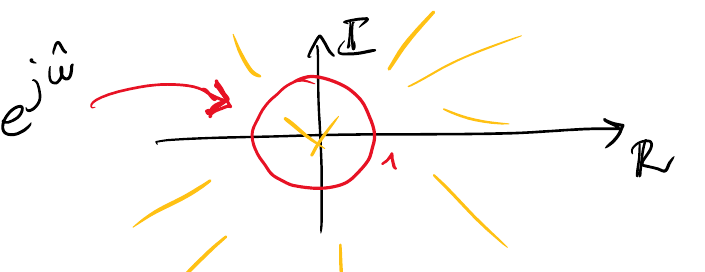
\includegraphics[scale=0.35]{immagini/lez26/trasformataZ.jpg}
\end{figure}

z e' quello che prima chiamavamo $e^{j \hat{\omega}}$, e grazie a questa generalizzazione notiamo che prima con la DTFT potevamo stare solamente sul cerchio unitario, in quanto $e^{j \hat{\omega}}$ valeva 1 in quei punti, mentre ora posso muovermi lungo tutto il piano (tranne dentro al cerchio).

\subsection{Esempio 1}

Consideriamo il seguente segnale e calcoliamone la trasformata Z:

\begin{figure}[ht!]
    \centering
    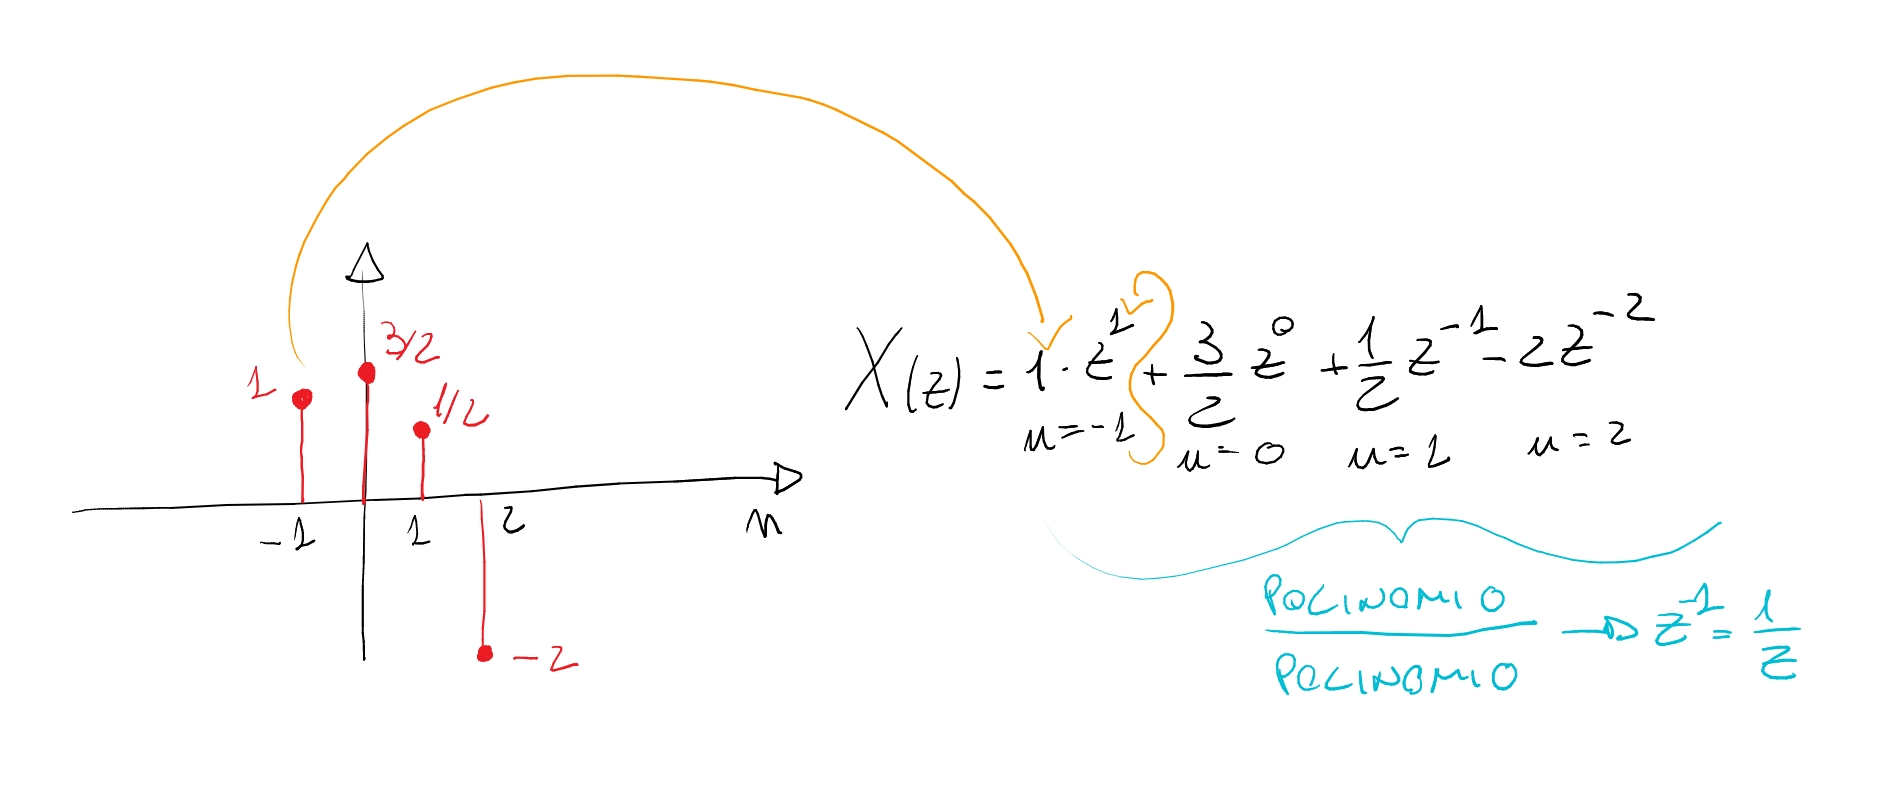
\includegraphics[scale=0.2]{immagini/lez26/es1TrasZ.jpg}
\end{figure}

Notiamo che abbiamo ottenuto tutti polinomi, diversamente da quanto succedeva con la DTFT dove ottenevamo una sommatoria di esponenziali complessi. Quindi possiamo dire che X(z) E' SEMPRE UN RAPPORTO DI DUE POLINOMI.

\subsection{Esempio 2}

Ora consideriamo il seguente segnale:

\[
x[n] = a^n u[n]
\]

Che ricordiamo esistere solo se $|a|<1$.

\begin{figure}[ht!]
    \centering
    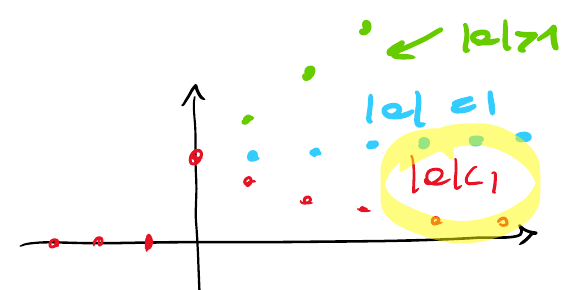
\includegraphics[scale=0.35]{immagini/lez26/esempio2.jpg}
\end{figure}

Troviamo la trasformata Z:

\[\begin{split}
    X(z) &= \sum_{n = -\infty}^{+\infty} a^n u[n] z^{-n} = \sum_{n=0}^{+\infty} (az^{-1})^n \\
    &\frac{1}{1 - az^{-1}} \mbox{ SE } |az^{-1}| < 1
\end{split}\]

$|az^{-1}| = \frac{|a|}{|z|} < 1 \leftarrow |z| > |a|$ e' molto importante e si chiama regione di convergenza ROC.

\begin{figure}[ht!]
    \centering
    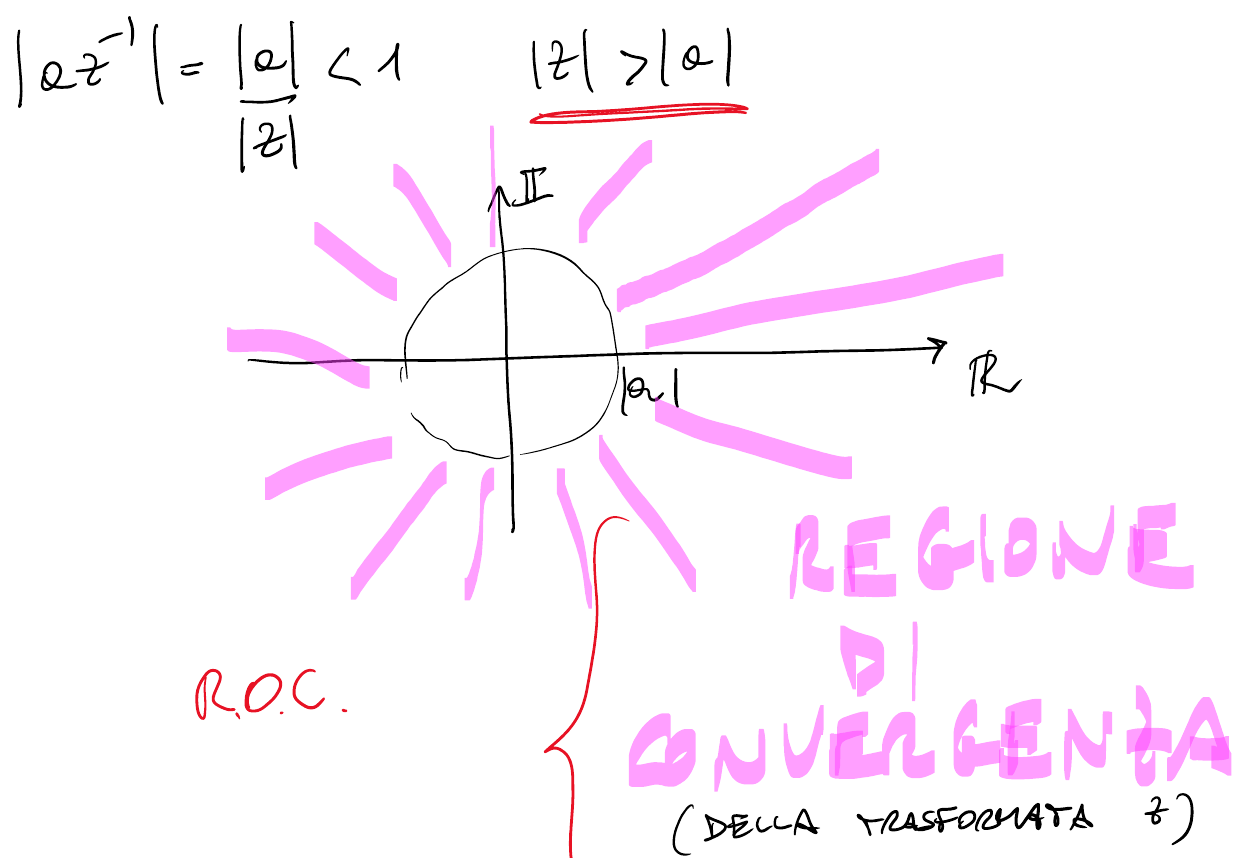
\includegraphics[scale=0.35]{immagini/lez26/regioneConvergenza.jpg}
\end{figure}

\newpage


\section{Trasformate note}
Vediamo due coppie di trasformate z (prese anche dagli esercizi che abbiamo fatto):

\[\begin{split}
    x[n] = a^n u[n] \leftrightarrow 
    \begin{cases}
    X(z) = \frac{1}{1 - a z^{-1}}\\
    R.O.C.: |z|>|a|\\
    \end{cases}\\
    x[n] = -a^n u[-n-1] \leftrightarrow 
    \begin{cases}
    X(z) = \frac{1}{1 - a z^{-1}}\\
    R.O.C.: |z|<|a|\\
    \end{cases}\\
\end{split}\]

Il primo e' chiamato gradino CAUSALE e notiamo che la sua ROC va verso infinito, mentre il secondo e' chiamato gradino ANTICAUSALE e la sua ROC va verso 0.

E' importante notare che, a differenza di quello che succedeva con la DTFT, la trasformata z non e' unica SE non la associamo alla sua ROC.
Possiamo quindi dire che $X(z) + ROC$ e' unica, quindi esiste un solo segnale di cui e' la trasformata z.

\section{Proprieta' della trasformata Z}
Vediamo ora tutte le proprieta' che ci serviranno della trasformata Z:

\subsection{Linearita'}

\[
    X(z) = \sum_{n = -\infty}^{+\infty} x[n] z^{-n}
\]

Notiamo che la trasformata z e' la composizione lineare di operatori lineari:
\begin{itemize}
    \item Somme
    \item Prodotti
    \item Costanti
\end{itemize}
Quindi e' anch'esso un operatore lineare.

\subsection{Ritardo temporale}
Questa e' una proprieta' molto importante per svolgere gli esercizi, vediamo cosa succede alla trasformata z quando ritardiamo il segnale di $n_0$ campioni:

\[\begin{split}
    x[n] &\leftrightarrow
    \begin{cases}
    X(z)\\
    R.O.C.\\
    \end{cases}\\
    x[n - n_0] &\leftrightarrow
    \begin{cases}
    X(z) \cdot z^{-n_0}\\
    R.O.C.
    \end{cases}
\end{split}\]

Vediamo che la trasformata e' moltiplicata per un fattore $z^{-n_0}$, dimostriamolo:

\[\begin{split}
    Z\{x[n-n_0]\} &= \sum_{n = -\infty}^{+\infty} x[n-n_0] z^{-n} \\
    \mbox{Cambio di variabile: } m &= n - n_0, n = m + n_0 \\
    &= \sum_{n = -\infty}^{+\infty} x[m] z^{-m -n_0} \\
    &=z^{-n_0} \sum_{m = -\infty}^{+\infty} x[m] z^{-m} = z^{-n_0} X(z)
\end{split}\]

\subsection{Convoluzione}
La convoluzione si trasforma in moltiplicazione:

\[
    x[n] * y[n] \leftrightarrow X(z) \cdot Y(z)
\]

\newpage

\subsection{ROC ha sempre simmetria radiale}
La trasformata z assume lo stesso valore per ogni $|z| = a$

\begin{figure}[ht!]
    \centering
    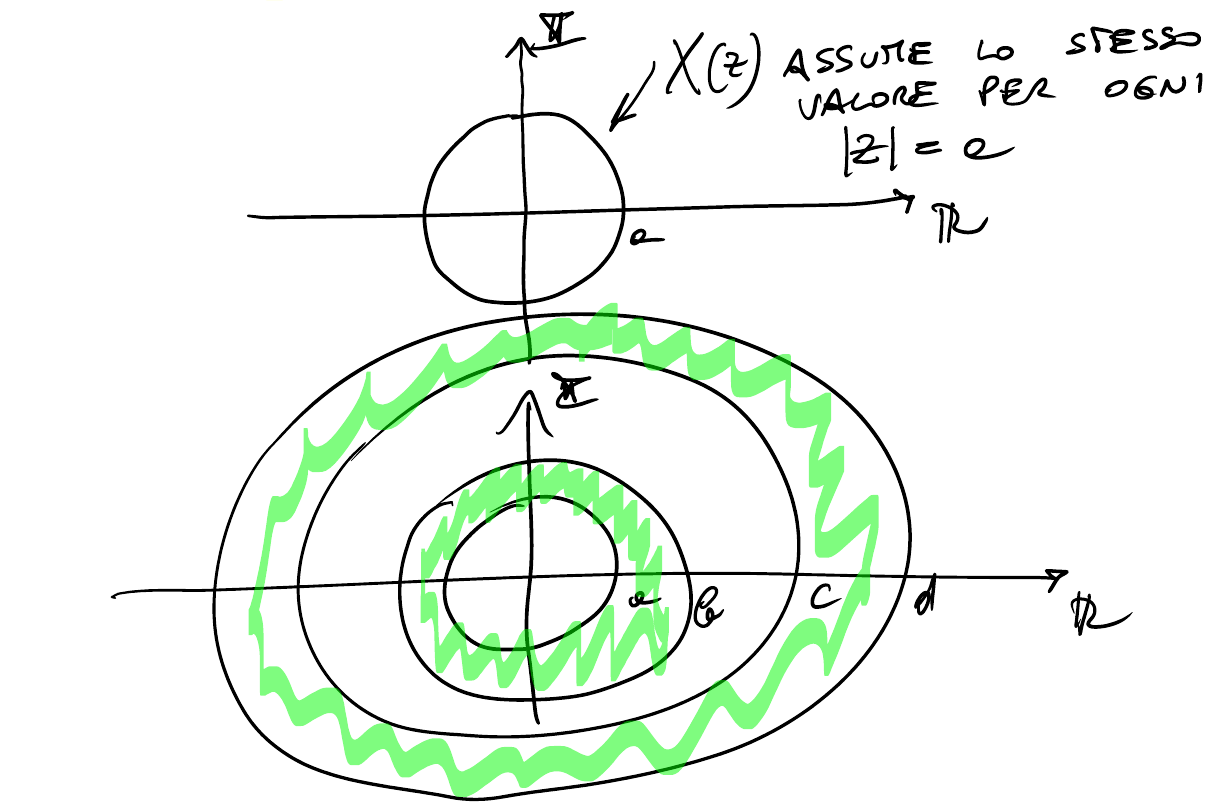
\includegraphics[scale=0.4]{immagini/lez27/ROCsimmetriaRadiale.jpg}
\end{figure}

Questo succede che la il modulo della trasformata z, che e' una sommatoria non deve divergere, ma notiamo che la trasformata dipende solo dal modulo, non dalla fase che invece puo' ruotare anche all'infinito ruotando intorno alla circonferenza, ed e' per questo che il $|X(z)|$ dipende solo dal modulo di z, che e' uguale su ogni circonferenza, con centro l'origine. Ne deriviamo quindi la simmetria radiale della ROC:

\[\begin{split}
    |X(z)| &= |\sum_{n = -\infty}^{+\infty} x[n] z^{-n}| \\
    &\le \sum_{n = -\infty}^{+\infty} |x[n] z^{-n}| = \sum_{n = -\infty}^{+\infty} |x[n]| |z^{-n}|
\end{split}\]
\newpage

\subsection{Nota a margine}
Negli schemi circuitali c'e' un segno particolare che e' il ritardo di un campione, che ha il simbolo del ritardo della trasformata z, non ha nulla a che vedere con la trasformata z, ma si rifa' alla sua proprieta' del ritardo temporale:

\begin{figure}[ht!]
    \centering
    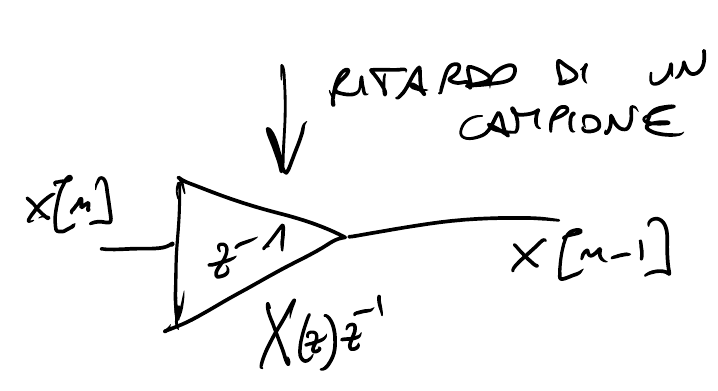
\includegraphics[scale=0.4]{immagini/lez27/notaMargine.jpg}
\end{figure}

\section{Funzione di trasferimento}

Partiamo ricordando qual'e' l'output di un sistema LTI:

\begin{figure}[ht!]
    \centering
    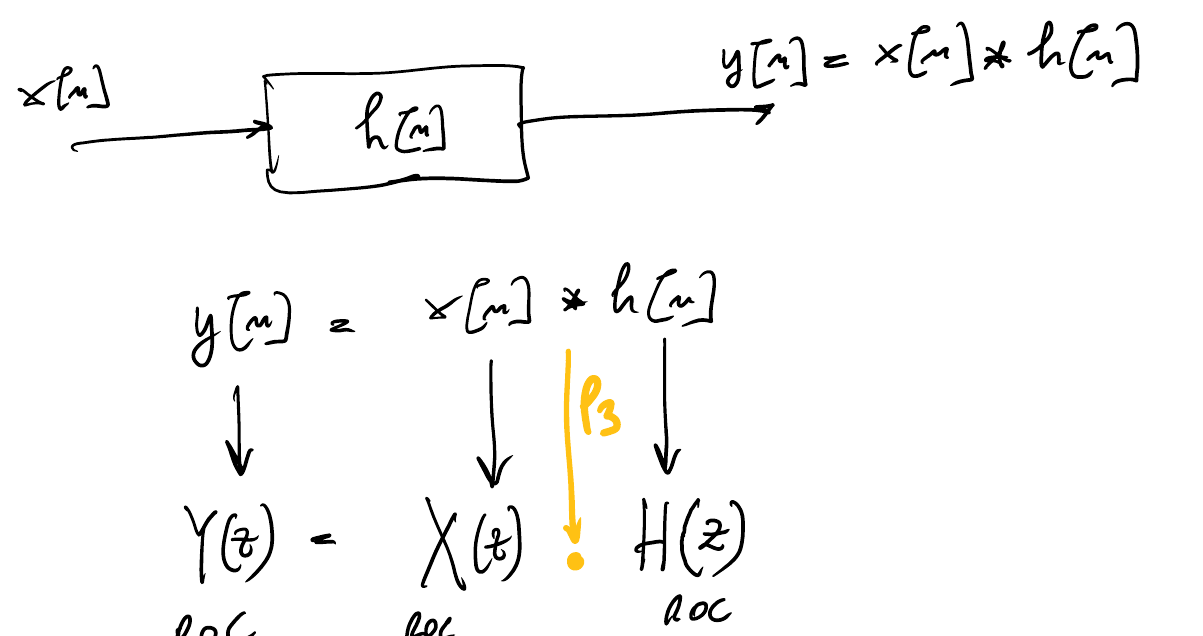
\includegraphics[scale=0.4]{immagini/lez27/funzioneTrasferimento.jpg}
\end{figure}

Vediamo che si facciamo la trasformata z di ogni elemento nell'equazione dell'uscita di un sistema LTI, applicando inoltre la proprieta' della trasformata che trasforma la convoluzione in moltiplicazione e successivamente raccogliamo la trasformata z della risposta all'impulso otteniamo la FUNZIONE DI TRASFERIMENTO:

\[
    Z\{h[n]\} = H(z) = \frac{Y(z)}{X(z)}
\]

E' chiamata funzione di trasferimento perche' trasferisce l'ingresso sull'uscita.

\subsection{$H(z)$ per un sistema LTI qualunque}

Vediamo ora come trovare la funzione di trasferimento partendo dall'equazione alle differenze di un sistema LTI qualunque, lo facciamo applicando le proprieta' che abbiamo appena visto:

\[\begin{split}
    &y[n] = \sum_{h = -N_1, h \neq 0}^{N_2} ah y[n-h] + \sum_{k = -M_1}^{M_2} bk x[n-k]\\
    &\mbox{Troviamo la trasformata z di ogni fattore ed applichiamo la proprieta' di linearita'}\\
    &Y(z) = \sum_{h = -N_1, h \neq 0}^{N_2} ah Z\{y[n-h]\} + \sum_{k = -M_1}^{M_2} bk Z\{x[n-k]\}\\
    &\mbox{Applichiamo la proprieta' del ritardo temporale per i segnali y e x:}\\
    &Y(z) = \sum_{h = -N_1, h \neq 0}^{N_2} ah Y(z) z^{-h} + \sum_{k = -M_1}^{M_2} bk X(z) z^{-k}\\
    &\mbox{Portiamo a sinistra i fattori che dipendono dalla trasformata Y:}\\
    &Y(z) - Y(z) \sum_{h = -N_1, h \neq 0}^{N_2} ah z^{-h} = X(z) \sum_{k = -M_1}^{M_2} bk  z^{-k}\\
    &\frac{Y(z)}{X(z)} = \frac{\sum_{k = -M_1}^{M_2} bk  z^{-k}}{\sum_{h = -N_1, h \neq 0}^{N_2} ah z^{-h}} = H(z)
\end{split}\]

E' importante notare che la funzione di trasferimento e' sempre una funzione razionale fratta (frazione tra due polinomi).

\section{Ripasso dell'algebra polinomiale}
Ricordiamo che un qualsiasi polinomio:
\[
    a_N z^N + a_{N-1}z^{N-1} +...+ a_1 z^1 + a_0 = 0
\]

Lo possiamo caratterizzare in due modi, o con i coefficienti:
\[
    a_0, a_1, a_2, ..., a_n
\]
Abbiamo quindi N+1 coefficienti.

Oppure fattorizzandolo (lo esprimiamo come prodotto di due o piu' fattori polinomiali di grado inferiore):
\[
    a_N(z - z_1)(z - z_2)...(z-z_N)
\]
Abbiamo quindi N radici appartenenti a C + un coefficiente ($a_n$).

Ricordiamo anche il teorema fondamentale dell'algebra che dice che per ogni polinomio di grado N ammette N soluzioni di C. Per ogni polinomio di grado N a coefficienti reali ammette N soluzioni reali o complesse coniugate.

\section{Zeri e Poli}
Riscriviamo la funzione di trasferimento di un generico sistema LTI fattorizzando i polinomi al numeratore ed al denominatore, notando che al numeratore abbiamo un polinomio di grado M, dove $M = M_1 + M_2$, mentre al denominatore abbiamo un polinomio di grado N, dove $N = N_1 + N_2$:

\[\begin{split}
    H(z) &= \frac{\sum_{k = -M_1}^{M_2} bk  z^{-k}}{\sum_{h = -N_1, h \neq 0}^{N_2} ah z^{-h}} \\
    &= \frac{b_M(z - z_1)(z-z_2) ... (z - z_M)}{a_N(z - p_1)(z-p_2) ... (z - p_N)}
\end{split}\]

e chiamiamo le radici $z_i$ del numeratore N(z) "ZERI", mentre chiamiamo le $p_i$ radici del denominatore D(z) "POLI".

\subsection{Esempio di zero}
Vediamo come si rappresenta una ZERO generico della funzione di trasferimento sul piano.
Consideriamo una generica trasformata z:

\[
    \epsilon(z) = |z - z_i|, z_i \in \mathbf{C}
\]

Possiamo inizialmente visualizzare il grafico di questa funzione immaginando che z e $z_i$ siano due vettori su un piano cartesiano, il modulo della differenza e' la distanza tra i due vertici del vettore, quindi possiamo dire che se z e' simile a $z_i$ (quasi coincidono) la funzione epsilon (ovvero il modulo della differenza) tendera' a 0, mentre se il modulo di z e' molto maggiore rispetto al modulo di $z_i$ possiamo dire che la funzione epsilon crescera' all'infinito.

\begin{figure}[ht!]
    \centering
    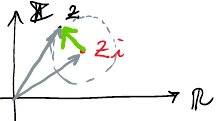
\includegraphics{immagini/lez28/zeroBidimensionale.jpg}
\end{figure}

Facciamo ora un ulteriore passo ricordandoci che la trasformata z gode della proprieta' di simmetria radiale, quindi in realta' la funzione epsilon sara' caratterizzata da tutti i punti sulla circonferenza centrata in $z_i$ con raggio la distanza tra $z_i$ e z.
Ora se aumentiamo di una dimensione il piano complesso, come avevamo detto avremmo fatto quando abbiamo iniziato a parlare della trasformata z, possiamo vedere che lo ZERO della funzione di trasferimento e' un cono centrato in $z_i$ (lo zero) che si allarga salendo lungo l'asse z (man mano che z aumenta).

\begin{figure}[ht!]
    \centering
    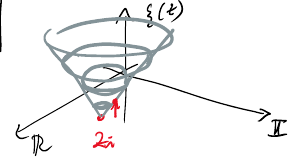
\includegraphics{immagini/lez28/zeroTridimensionale.jpg}
\end{figure}

\section{Esempi}
Vediamo adesso una serie di esempi, ma prima diamo la definizione di PRODUTTORIA, che ci serve per poter riscrivere la funzione di trasferimento. Produttoria:

\[
    \prod_{i = 1}^{N} x_i = x_1 \cdot x_2 \cdot x_3 \cdot x_4 ... \cdot x_N
\]


\[
    |H(Z)| = |\frac{b_M \prod_{i = 1}^M (z - z_i)}{a_N \prod_{j = 1}^N (p - p_j)}| = \frac{|b_M| \prod_{i = 1}^M |z - z_i|}{|a_N| \prod_{j = 1}^N |p - p_j|}
\]

Da questa definizione possiamo vedere delle caratteristiche degli ZERI, dato che il denominatore sara' piccolo quando siamo vicini ad uno zero, gli zeri tendono a far diventare piccola la funzione di trasferimento, graficamente possiamo immaginarlo come se schiacciassimo la funzione sul piano orizzontale.
Mentre per quanto riguarda i POLI, notiamo che NON possono essere nella regione di convergenza, perche' il denominatore della funzione di convergenza andrebbe a 0, quindi tutto tenderebbe ad infinito, questa cosa graficamente possiamo immaginarla come se i poli alzassero verso infinito la funzione, come un paletto che alza la tenda.

\subsection{Esempio 1}

Cominciamo da un esempio semplice, consideriamo:

\[
    H(z) = 1
\]

\newpage

Vediamo subito il grafico di questa funzione di derivazione:

\begin{figure}[ht!]
    \centering
    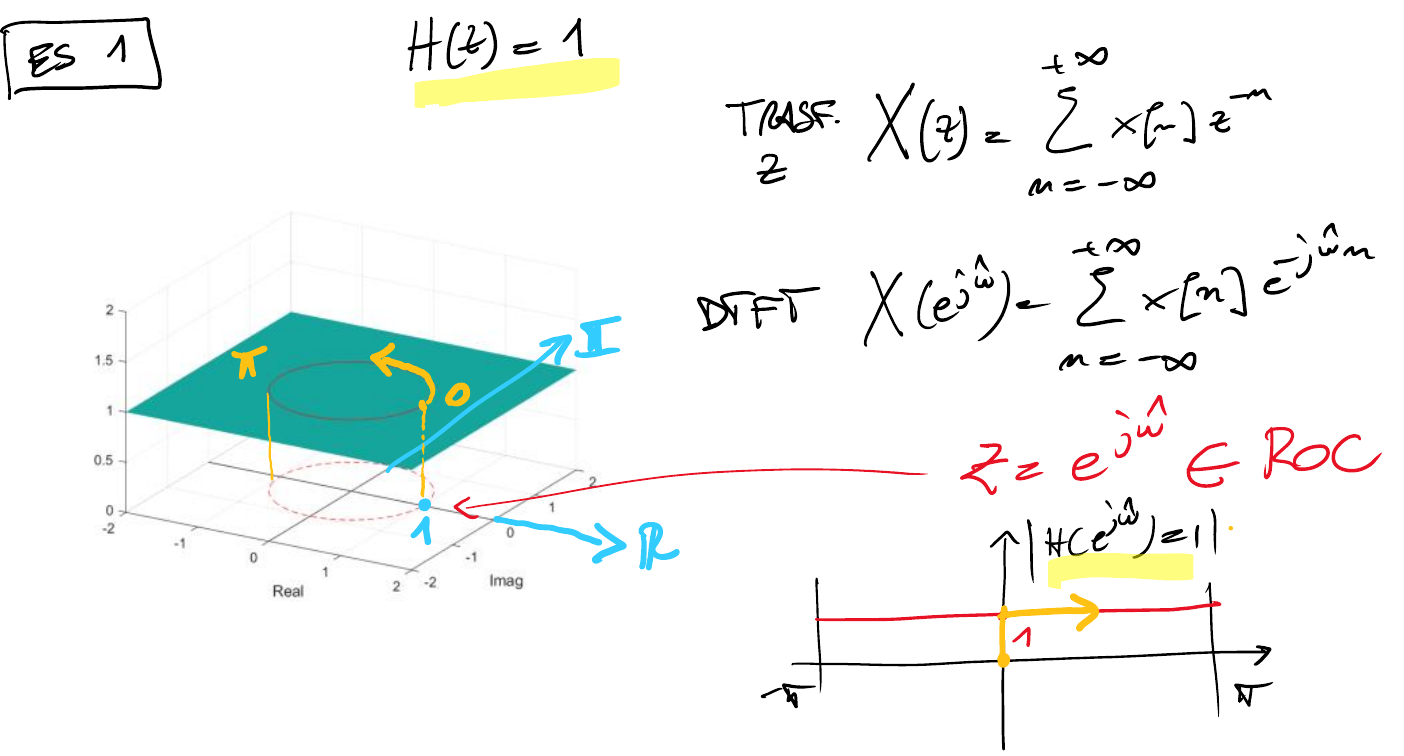
\includegraphics[scale=0.4]{immagini/lez28/es1.jpg}
\end{figure}

Vediamo che la funzione di trasferimento e' il piano verde, che e' un piano infinito che sta sopra al piano complesso, e' cosi' perche' ad ogni valore questa funzione associa 1.

Il cerchio invece e' la proiezione del cerchio unitario (la DTFT), quindi e' come se avessi trovato la risposta in frequenza del sistema che e' 1, e poi partendo dal punto 1 sul piano complesso, che corrisponde alla frequenza 0 sul grafico del modulo mi spostassi sul cerchio unitario. Facendo questa cosa posso riportare il movimento sul grafico del modulo dela risposta in frequenza.
Notiamo che lo possiamo fare perche' il cerchio unitario appartiene alla ROC della trasformata z.

\subsection{Esempio 2}
Ora vediamo una funzione di trasferimento piu' complessa:

\[
    H(z) = z - \frac{1}{2}
\]

Che notiamo essere nella forma $\varepsilon(z) = |z - z_i|$ e sappiamo gia' che il grafico di questa funzione di trasferimento e' un cono puntato in $z_i$, in questo caso in $\frac{1}{2}$, quindi possiamo dire che $\frac{1}{2}$ e' uno ZERO della funzione di trasferimento.

Ora dato che il cerchio unitario appartiene alla ROC, possiamo sostituire $z = e^{j \hat{\omega}}$ per trovare la risposta in frequenza:

\[
    H(e^{j\hat{\omega}}) = e^{j \hat{\omega}} - \frac{1}{2}
\]

Ora per disegnare il grafico del modulo della risposta in frequenza possiamo farlo in modo spannometrico guardando la proiezione del cerchio unitario sulla trasformata z. Ci poniamo inizialmente nel punto 1 sulla proiezione del cerchio unitario, che ricordiamo coincidere alla frequenza 0 nel grafico del modulo della risposta all'impulso, notiamo subito che e' il punto con altezza minore rispetto al piano complesso, non sappiamo esattamente quant'e', ma possiamo approssimarlo. Successivamente cominciamo a muoverci sul cerchio di raggio unitario fino ad arrivare al punto -1, che corrisponde alla frequenza $\pi$, notiamo che l'altezza dei punti che stiamo percorrendo rispetto al piano complesso aumenta fino al punto -1, e riportiamo questa informazione sul grafico del modulo.
Per disegnare il modulo da 0 a $-\pi$ semplicemente ribaltiamo lungo l'asse y la parte che abbiamo trovato tra 0 e $+\pi$.


\begin{figure}[ht!]
    \centering
    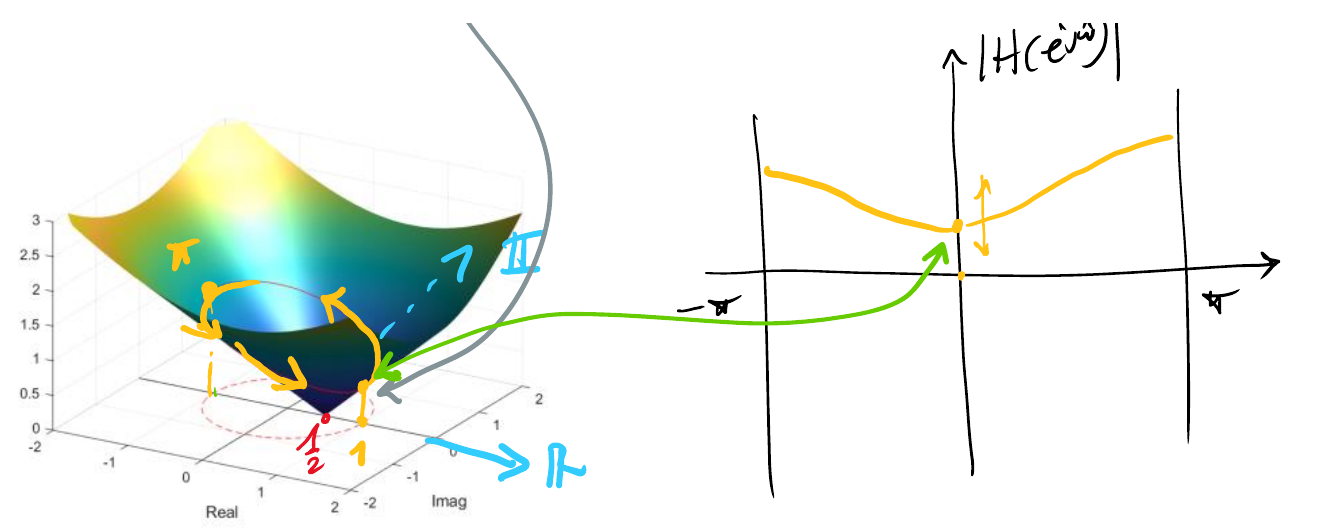
\includegraphics[scale=0.4]{immagini/lez28/es2.jpg}
\end{figure}

\subsection{Esempio 3}

Ora consideriamo:

\[
    H(z) = \frac{1}{z - \frac{1}{3}}
\]

Notiamo subito che il punto $\frac{1}{3}$ non appartiene alla ROC, perche' porterebbe il denominatore a 0, quindi e' un POLO, sappiamo quindi che il cerchio centrato nell'origine con raggio $\frac{1}{3}$ non appartiene alla ROC, questo potrebbe essere un problema perche' dobbiamo capire se il cerchio unitario appartiene alla ROC, in questo caso non abbiamo problemi perche' la funzione di trasferimento appartiene ad un gradino causale, sappiamo quindi che la ROC esiste per valori di z maggiori di a, quindi si estende da $\frac{1}{3}$ a $+\infty$.
Comunque possiamo sostituire $z = e^{j \hat{\omega}}$ in quanto il cerchio di raggio unitario appartiene alla ROC:

\[
    H(e^{j\hat{\omega}}) = \frac{1}{e^{j\hat{\omega}} - \frac{1}{3}}
\]

Per costruire il grafico del modulo della risposta in frequenza faccio come prima, mi porto nel punto 1 (che corrisponde alla frequenza 0) e mi muovo lungo la proiezione del cerchio unitario.

La cosa interessante di questo esempio e' vedere cosa succede quando e' presente un POLO, come abbiamo detto in precedenza il polo porta verso infinito la funzione. Per indicare la presenza di POLI e ZERI possiamo costruire un grafico POLI-ZERI, in cui indico con una X la presenza di un polo e con uno 0 la presenza di uno ZERO.

\begin{figure}[ht!]
    \centering
    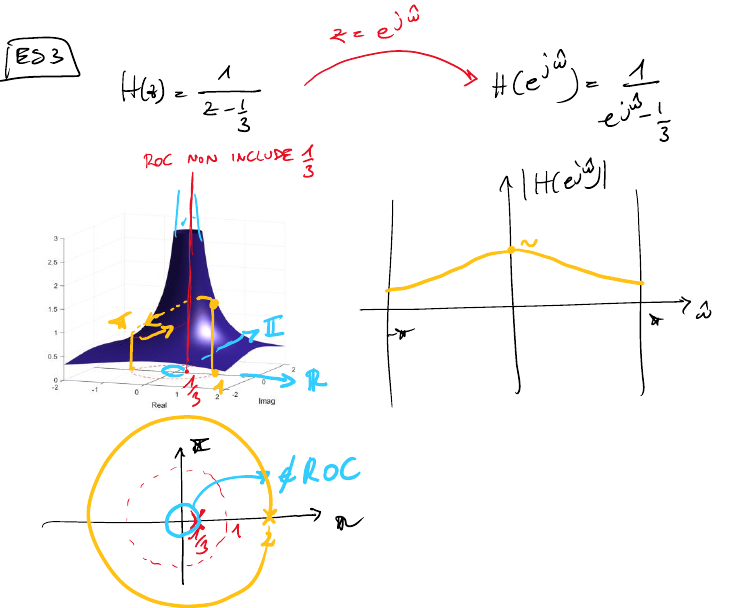
\includegraphics[scale=0.7]{immagini/lez28/es3.jpg}
\end{figure}

\newpage
\section{Dalla $H(z)$ all'equazione alle differenze}

Non abbiamo ancora visto qual'e' l'equazione alle differenze che genera la $H(z)$. Dobbiamo usare la trasformata z inversa: $z^{-1}$, ma non vedremo nessuna formula, useremo le coppie di trasformate z note.

Vediamolo per ogni esempio che abbiamo visto.

Esempio 1:

\[\begin{split}
    \frac{Y(z)}{X(z)} &= H(z) = 1\\
    Y(z) &= X(z)\\
    y[n] &= x[n]
\end{split}\]

Esempio 2:
\[\begin{split}
    \frac{Y(z)}{X(z)} &= H(z) = z - \frac{1}{2}\\
    Y(z) &= X(z) z^{-(-1)} - \frac{1}{2}X(z)\\
    y[n] &= x[n+1] -\frac{1}{2}x[n]
\end{split}\]

Abbiamo trovato un equazione FIR anticausale

Esempio 3:

\[\begin{split}
    \frac{Y(z)}{X(z)} &= H(z) = \frac{1}{z - \frac{1}{3}}\\
    Y(z) z - Y(z)\frac{1}{3} &= X(z)\\
    y[n+1] - \frac{1}{3}y[n] &= x[n]\\
    y[n] &= 3y[n+1] - 3x[n]
\end{split}\]

Abbiamo trovato un equazione IIR anticausale.

\section{Da $H(z)$ alla risposta all'impulso}
Se faccio la trasformata z inversa direttamente della funzione di trasferimento, trovo la risposta all'impulso. Lo facciamo sempre guardando le trasformate note.

Vediamo applicato a tutti gli esempi che abbiamo visto.

Esempio 1:

\[\begin{split}
    H(z) &= 1\\
    h[n] &= \delta[n]
\end{split}\]

Esempio 2:

\[\begin{split}
    H(z) &= z - \frac{1}{2} \\
    h[n] &= \delta[n + 1] - \frac{1}{2} \delta[n]
\end{split}\]

Esempio 3:

\[\begin{split}
    H(z) &= \frac{1}{z-\frac{1}{3}} = \frac{z^{-1}}{1 - \frac{1}{3} z^{-1}} \\
    &= \frac{1}{1 - \frac{1}{3} z^{-1}} \cdot z^{-1}
\end{split}\]

Qui pero' abbiamo un problema, perche' non sappiamo se e' un sistema causale o anticausale, ed il comportamento del gradino cambia in base al tipo di sistema, quindi se ROC: $|z| > |\frac{1}{3}$|, allora $h[n] = (\frac{1}{3})^{n-1} u[n-1]$.
Invece se ROC: $|z| < |\frac{1}{3}|$, allora $h[n] = -(\frac{1}{3})^{n-1} u[-(n-1)]$.

\newpage

\section{Esempio 4}
Partiamo adesso da un filtro causale FIR:

\[
    y[n] = x[n] - \sqrt{2} x[n-1] + x[n-2]
\]  

Da cui voglio ricavare il grafico del modulo della risposta in frequenza.
Per farlo ho a disposizione due procedure, una e' quella che usavamo fino ad adesso, ovvero troviamo la risposta all'impulso, da cui ricaviamo tramite la formula la risposta in frequenza, poi ci riconduciamo alla forma con il coseno e disegniamo il modulo del coseno.
Facciamolo:

\[\begin{split}
    h[n] &= \delta[n] - \sqrt{2} \delta[n-1] + \delta[n-2]\\
    H(e^{j\hat{\omega}}) &= 1 - \sqrt{2} e^{-j \hat{\omega}} + e^{-j 2 \hat{\omega}} \\
    &= 2e^{-j\hat{\omega}} \{\frac{e}{2}^{j\hat{\omega}} - \frac{\sqrt{2}}{2} + \frac{e}{2}^{-j\hat{\omega}}\} \\
    &= 2(\cos\hat{\omega} - \frac{\sqrt{2}}{2}) e^{-j\hat{\omega}}
\end{split}\]

\begin{figure}[ht!]
    \centering
    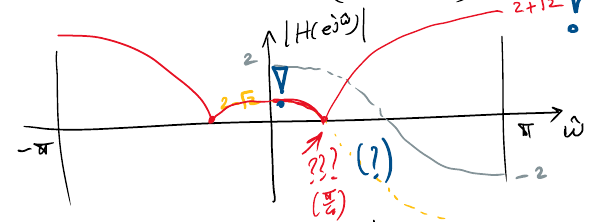
\includegraphics[scale=0.7]{immagini/lez28/es4.jpg}
\end{figure}

Utilizziamo adesso una seconda procedura trovando la funzione di trasferimento del sistema, successivamente trovare i zeri ed i poli della funzione, disegnare il grafico poli-zeri e da quello trovare il grafico approssimativo del modulo della risposta in frequenza.
Facciamolo:

\[\begin{split}
    &y[n] = x[n] - \sqrt{2} x[n-1] + x[n-2]\\
    &\mbox{Usiamo subito la proprieta' di linearita'}\\
    &Y(z) = X(z) - \sqrt{2} Z\{x[n-1]\} + Z\{x[n-2]\} \\
    &\mbox{Usiamo la proprieta' del ritardo}\\
    &Y(z) = X(z) - \sqrt{2} X(z) z^{-1} + X(z) z^{-2}\\
    &\frac{Y(z)}{X(z)} = 1 - \sqrt{2} z^{-1} + z^{-1} = \frac{z^2 - \sqrt{2}z + 1}{z^2}
\end{split}\]

Dobbiamo trovare gli ZERI:

\[\begin{split}
    &z^2 - \sqrt{2}z + 1 = 0 \\
    &Z_{1,2} = \frac{\sqrt{2} \pm \sqrt{2-4}}{2} = \frac{\sqrt{2} \pm i \sqrt{2}}{2} = \sqrt{\frac{2}{4} + \frac{2}{4}} e^{\pm i \frac{\pi}{4}}
\end{split}\]

ed i POLI:

\[
    p_1 = p_2 = 0
\]

\begin{figure}[ht!]
    \centering
    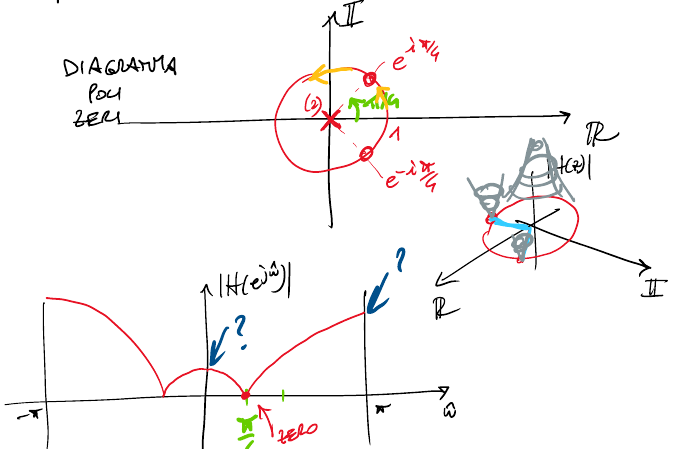
\includegraphics[scale=0.7]{immagini/lez28/es4v2.jpg}
\end{figure}

Quello che faccio e' disegnare inizialmente il diagramma poli zeri, poi lo uso per fare il grafico del modulo percorrendo la circonferenza del cerchio unitario da 1 a $\pi$. Da questo esempio possiamo notare che quando ho uno zero che e' sul cerchio, nel grafico del modulo quei punti vanno a zero, quindi e' come se stessi tagliando quelle frequenza, nel nostro esempio quelle a $\frac{\pi}{4}$.

\section{Esercizio}
Facciamo un esercizio un po' piu' complicato, data la seguente funzione di trasferimento:

\[
    H(z) = \frac{1 - \sqrt{3}z^{-1} + z^{-2}}{1 - 0,9 \sqrt{3} z^{-1} + 0,81 z^{-2}} = \frac{Y(z)}{X(z)}
\]  

Vogliamo trovare l'equazione alle differenze che l'ha generata. Per farlo dobbiamo fare la trasformata z inversa di Y(z) e X(z):

\[\begin{split}
    &X(z)[1 - \sqrt{3}z^{-1} + z^{-2}] = Y(z)[1 - 0,9 \sqrt{3} z^{-1} + 0,81 z^{-2}]\\
    &X(z) - \sqrt{3}z^{-1}X(z) + X(z) + z^{-2} = Y(z) - 0,9 \sqrt{3}z^{-1} Y(z) + 0,81z^{-2}Y(z)\\
    &\mbox{Facciamo la trasformata inversa}\\
    &x[n] - \sqrt{3} x[n-1] + x[n-2] = y[n] - 0,9 \sqrt{3} y[n-1] + 0,81 y[n-2]\\
    &y[n] = 0,9 \sqrt{3}y[n-1] - 0,81 y[n-2] + x[n] - \sqrt{3} x[n-1] + x[n-2]
\end{split}\]

Ora vogliamo disegnare il diagramma poli-zeri, desumendo un grafico approssimativo della risposta in frequenza, e dire che filtro e'.

Il consiglio e' di considerare sempre i polinomi con esponenti negativi, ma quando dobbiamo trovare i poli e gli zeri di portarli in positivo, per farlo in questo caso raccogliamo la potenza negativa maggiore sia al numeratore che al denominatore:

\[\begin{split}
    H(z) &= \frac{1 - \sqrt{3}z^{-1} + z^{-2}}{1 - 0,9 \sqrt{3} z^{-1} + 0,81 z^{-2}}\\
    &= \frac{z^{-2}(z^2 - \sqrt{3}z + 1)}{z^{-2}(z^2 - 0,9 \sqrt{3}z + 0,81)}
\end{split}\]

ora calcoliamo gli ZERI, portandoli in forma polare:
\[
    Z_{1,2} = \frac{\sqrt{3} \pm \sqrt{3-4}}{2} = \frac{\sqrt{3}}{2} \pm i\frac{1}{2} = e^{\pm i \frac{\pi}{3}}
\]

e i POLI, portandoli in forma polare:
\[
    P_{1,2} = \frac{0,9\sqrt{3}\pm \sqrt{0,81 \cdot 3 - 0,81 \cdot 4}}{2} = \frac{0,9 \sqrt{3} \pm 0,9 i}{2} = 0,9 (\frac{\sqrt{3}}{2} + \frac{1}{2}i) = e^{i \frac{\pi}{3}}
\]
\newpage

Ora riportiamo i poli e gli zeri nel grafico poli-zeri e come fatto in precedenza percorrendo il cerchio unitario disegniamo il grafico del modulo della risposta in frequenza.

\begin{figure}[ht!]
    \centering
    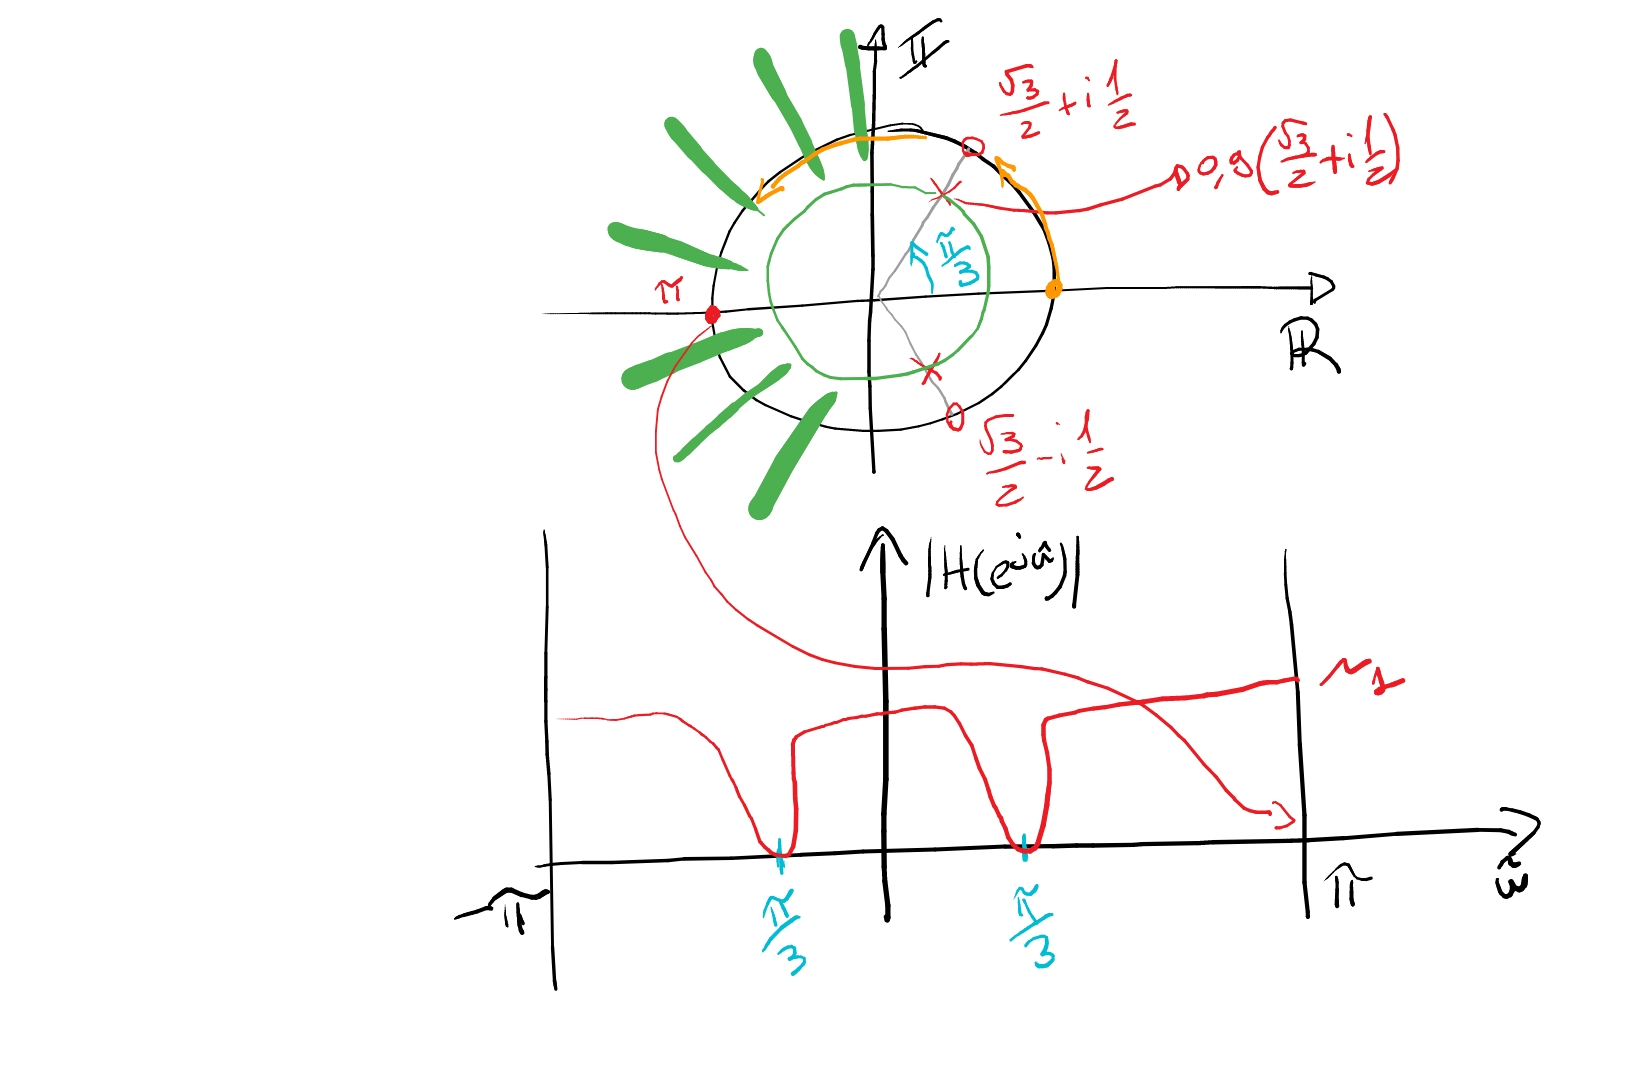
\includegraphics[scale=0.3]{immagini/lez29/graficoEs.jpg}
\end{figure}

\[
    z = e^{j \hat{\omega}} \in ROC \leftarrow X(z) = \frac{1 - \sqrt{3} e^{j\hat{\omega}} + e^{-j\hat{\omega}2}}{1 - 0,9 \sqrt{3} e^{-j\hat{\omega}} + 0,81 e^{-j 2 \hat{\omega}}} = H(e^{j\hat{\omega}})
\]

Una cosa da notare di questo esercizio e' che i poli o gli zeri posti all'origine degli assi non fanno niente, quindi possiamo non considerarli.
Questo filtro si chiama blocca banda.

\section{Esercizio}
Data la seguente funzione di trasferimento:

\[
    H(z) = \frac{1}{1 - 2 z^{-1}} + \frac{1}{1 - \frac{1}{3} z^{-1}}
\]

Ci viene detto che la ROC e' $\frac{1}{3} < |z| < 2$, vogliamo trovare la risposta in frequenza $h[n]$.

Per farlo dobbiamo applicare la trasformate z inversa, ma prima disegniamo il grafico poli-zeri per capire se il sistema e' causale o anticausale e capire che trasformata nota dobbiamo usare.

Gli zeri non li posso calcolare (o meglio dovrei fare il denominatore comune e trovare i numeratori), sappiamo pero' che i poli sono quelli che annullano i due denominatori,
quindi per il primo denominatore:

\[\begin{split}
    1 -2z^{-1} = 0 \\
    z^{-1} = \frac{1}{2}\\
    z = 2
\end{split}\]

per il secondo:
\[\begin{split}
    1 - \frac{1}{3} z^{-1} = 0\\
    z^{-1} = 3 \\
    z = \frac{1}{3}
\end{split}\]

Notiamo che i poli di polinomi di questo tipo sono sempre i numeri che moltiplicano la z.

\begin{figure}[ht!]
    \centering
    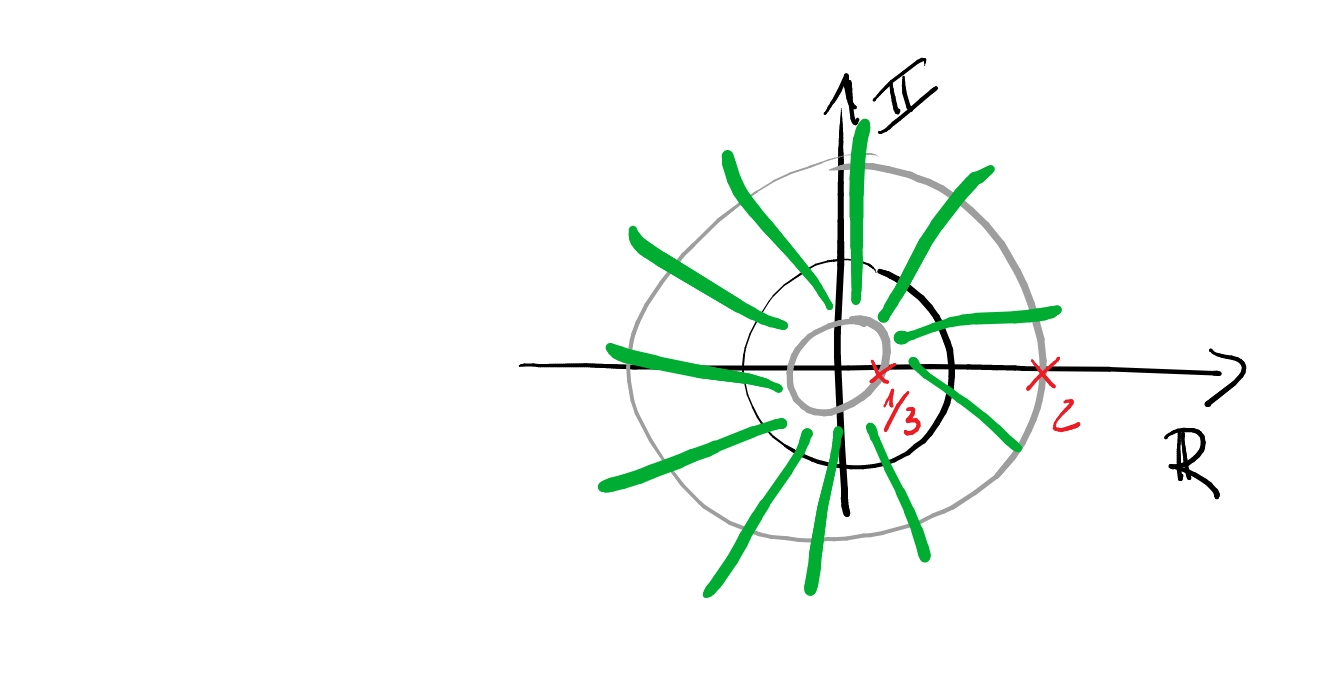
\includegraphics[scale=0.2]{immagini/lez29/poliZeriEsercizio.jpg}
\end{figure}

Quindi da questo grafico capiamo che per il primo polinomio dobbiamo usare il gradino anticausale, perche' la ROC e' minore di 2, quindi va verso l'interno. Al contrario per il secondo polinomio dobbiamo usare il gradino causale, perche' la ROC va da $\frac{1}{3}$ verso l'esterno.

\[\begin{split}
    h[n] &= Z^{-1} \{\frac{1}{1 - 2z^{-1}}\} + Z^{-1} \{\frac{1}{1 - \frac{1}{3} z^{-1}}\} \\
    h[n] &= -2^n u[-n-1] + (\frac{1}{3})^n u[n]
\end{split}\]

\section{All zeros, All poles}

Troviamo ora un collegamento tra filtri FIR, IIR e la loro quantita' di poli e zeri.

\begin{figure}[ht!]
    \centering
    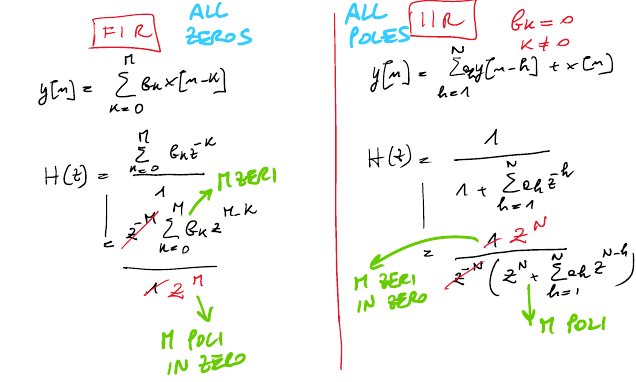
\includegraphics[scale=0.7]{immagini/lez29/allZeroAllPoles.jpg}
\end{figure}

Notiamo che i filtri FIR hanno M zeri e 0 poli, o meglio hanno M poli tutti in zero che come abbiamo visto in precedenza non contano. Viceversa i filtri IIR hanno M poli e M zeri tutti in zero (quindi non contano).

\section{Esempio}
Vediamo un esercizio che ci permettera' di introdurre una tecnica per calcolare la trasformata z inversa, la tecnica dei residui.

Partiamo da un equazione alle differenze causale:

\[
    y[n] = a_1 y[n-1] + b_0 x[n]
\]

Vogliamo ora calcolare l'uscita di questo sistema $y[n]$ se mettiamo in input:

\[
    x[n] = u[n]
\]

Quello che avremmo dovuto fare prima della trasformata Z era calcolare la convoluzione tra il sistema ed il segnale in input. 
Ma ora possiamo calcolare la funzione di trasferimento del sistema, la trasformata z del segnale e fare la moltiplicazione (propritea' della convoluzione) tra le due trasformate, successivamente fare la trasformata inversa del risultato trovando cosi' $y[n]$.

Quindi inizialmente calcoliamo la funzione di trasferimento $H(z)$ dell'equaazione alle differenze:

\[\begin{split}
    y[n] = a_1 y[n-1] + b_0 x[n]\\
    Y(z) = a_1 Y(z) z^{-1} + b X(z)\\
    Y(z) \{1 - a_1 z^{-1}\} = bX(z)\\
    \frac{y(z)}{X(z)} = \frac{b}{1 - a_1 z^{-1}} = H(z)
\end{split}\]

Della funzione di trasferimento possiamo dire che la ROC e' $|z| > |a|$, perche' sapevamo che il sistema che l'ha generata e' causale, inoltre esiste un solo polo che e' $a_1$.

Ora troviamo la trasformata z del segnale in input:

\[
    x[n] = u[n] \leftarrow \frac{1}{1 - z^{-1}} = X(z)
\]

Dato che e' un esponenziale causale (gradino causale) la ROC e' $|z| > 1$.

Ora facciamo la moltiplicazione tra le due trasformate che abbiamo trovato:

\[
    Y(z) = H(z) \cdot X(z) = \frac{b}{1 - a_1 z^{-1}} \cdot \frac{1}{1 - z^{-1}}
\]

Per trovare la ROC dobbiamo trovare qual'e' la condizione piu' stringente tra le ROC di ogni trasformata. Il problema diceva anche che $a_1 < 1$, quindi la condizione piu' stringente tra le due ROC e' $|z| > 1$. Inoltre abbiamo due poli, uno in $p_1 = 1$ e l'altro in $p_2 = a_1$.
Tracciamo il grafico poli-zeri:

\begin{figure}[ht!]
    \centering
    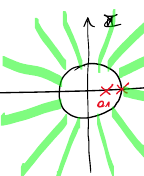
\includegraphics[scale=0.7]{immagini/lez29/poliZeroEs.jpg}
\end{figure}

Ora per trovare $Y(z)$ abbiamo due strategie, possiamo portare a denominatore comune le due frazioni e cercare in numeratori corretti:

\[\begin{split}
    Y(z) = \frac{b}{(1 - a_1 z^{-1})(1 - z^{-1})} = \frac{B_1}{(1 - a_1 z{-1}} + \frac{B_2}{(1 - z^{-1})}
\end{split}\]

Devo trovare i valori di $B_1$ e $B_2$, per farlo basta risolvere questo sistema:

\[\begin{split}
    &\begin{cases}
    B_1 + B_2 = b \\
    -B_1 - a_1B_2 = 0
    \end{cases}\\
    &B_2 - a_1B_2 = b\\
    &B_2 = \frac{b}{1 - a_1}\\
    &B_1 = b - B_2 = \frac{\cancel{b} -b a_1 \cancel{-b}}{1 - a_1}
\end{split}\]

da cui:

\[\begin{split}
    &\frac{B_1(1 - z^{-1}) + B_2(1-a_1 z^{-1})}{(1 - a_1 z^{-1})(1 - z^{-1})}\\
    &\frac{b}{1-a_1} \cdot \frac{1}{1-z^{-1}} - \frac{ba_1}{1 - a_1} \cdot \frac{1}{1 - a_1 z^{-1}}
\end{split}\]

e dato che il sistema e' causale otteniamo:

\[
    y[n] = \frac{b}{1 - a_1} u[n] - \frac{b a_1}{1 - a_1} a_1^n u[n]
\]

Oppure potevamo usare la TECNICA DEI RESIDUI, ma prima di utilizzarla dobbiamo fare 3 verifiche (altrimenti lasciamo stare):
\begin{enumerate}
    \item Il polinomio deve essere espresso in potenze negative $z^{-k}$
    \item I poli sono singoli, hanno molteplicita' 1 (non devono esserci due poli coincidenti in un punto solo)
\end{enumerate}

Quello che dobbiamo fare per trovare $B_1$ e $B_2$ e' moltiplicare la frazione per un fattore che cancella il polo (opposto del fattore che genera il polo), quindi:

\[\begin{split}
    B_1 &= [Y(z) \cdot(1 - p_1z^{-1})] = [\frac{b}{\cancel{(1 - a_1 z^{-1})}(1 - z^{-1})} \cdot \cancel{(1 - a_1 z^{-1})}] = \frac{b}{1 - a^{-1}} \\
    B_2 &= [Y(z) \cdot(1 - p_1z^{-1})] = [\frac{b}{(1 - a_1 z^{-1}) \cancel{(1 - z^{-1})}} \cdot \cancel{(1 - z^{-1})}] = \frac{b}{1 - a_1} \\
\end{split}\]

\section{Metodo dei residui}
Formalizziamo meglio il metodo dei residui che abbiamo appena visto.
Partiamo da una funzione di trasferimento, che come abbiamo gia' visto e' una funzione razionale fratta, per cui sappiamo che il numeratore e' un polinomio espresso in potenze negative di z, mentre il denominatore lo definiamo come una produttoria di poli della funzione di trasferimento. Il metodo dei residui ci serve per trovare la risposta all'impulso del sistema partendo dalla funzione di trasferimento.

\[\begin{split}
    H(z) &= \frac{N(z^{-1})}{\prod_{h=1}^{N} R_h \cdot \frac{1}{1 - p_h z^{-1}}}
\end{split}\]

Quello che facciamo quindi nel metodo dei residui e' trasformare la produttoria in una sommatoria in cui moltiplichiamo la funzione di trasferimento per un RESIDUO che mi serve per annullare lo zero della funzione.

Prima di applicare questa tecnica devo fare delle verifiche:
\begin{enumerate}
    \item Assicurarsi che i polinomi siano espressi in $z^{-1}$
    \item Assicurarsi che i poli siano semplici, ovvero che non abbiamo molteplicita' diversa da 1.
    \item Se il grado del numeratore e' minore del grado del denominatore. Se non lo fosse bisogna fare la divisione tra polinomi per abbassare i gradi dei polinomi.
\end{enumerate}

\[
R_h = [H(z)(1 - p_h z^{-1})]
\]

\section{Stabilita' di un filtro LTI}

Cosa intendiamo con stabilita' di un sistema.
Parliamo di stabilita' B.I.B.O (Bounded Input Bounded Output), che semplicemente ci dice che se in un sistema LTI mettiamo in input un segnale finito ci aspettiamo in output un segnale finito.

\begin{figure}[ht!]
    \centering
    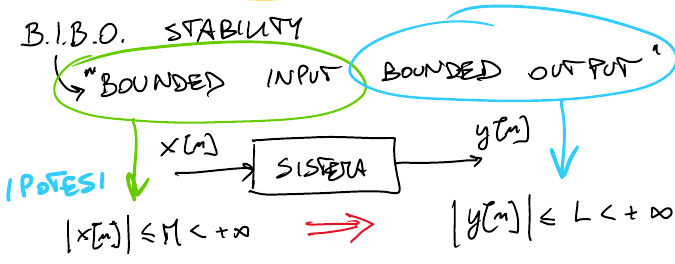
\includegraphics[scale=0.7]{immagini/lez30/BIBO.jpg}
\end{figure}

Un esempio semplice di una situazione che viola questa stabilita' e' ad esempio una cantante che fa scoppiare i bicchieri con la voce. La voce e' un input limitato che entrando in un sistema, il bicchiere, produce un output illimitato che fa scoppiare i bicchieri.
Un esempio piu' vicino all'elaborazione dei segnali e' quando un segnale satura e fischia.

\subsection{Teorema 1}
Dato un sistema LTI, condizione necessaria e sufficiente per la BIBO stabilita' e' che la risposta all'impulso sia assolutamente sommabile:

\[
    \sum_{n = -\infty}^{+\infty} |h[n]| < + \infty
\]

Dimostriamo la parte sufficiente:

Se LTI $ \sum_{n = -\infty}^{+\infty} |h[n]| < + \infty$ allora il sistema LTI e' stabile

\[\begin{split}
    y[n] &= x[n] * h[n] = \sum_{k = -\infty}^{+\infty} h[k] x[n-k]\\
    |y[n]| &= |\sum_{k = -\infty}^{+\infty} h[k] x[n-k]| \le \sum_{k = -\infty}^{+\infty} |h[k] x[n-k]| \\
    &= \sum_{k = -\infty}^{+\infty} |h[k]| |x[n-k]| \le \sum_{k = -\infty}^{+\infty} |h[k]| \cdot M \\
    &= M \sum_{k = -\infty}^{+\infty} h[k] = M \Tilde{h}\\
    |y[n]| &\le M \Tilde{h} < +\infty
\end{split}\]
